\chapter{PLACEMENT OF FIGURES IN \LaTeX }\label{chap2:body1}


When creating figures in \LaTeX, it is important to realize that
different types of figures are imported differently, leading to
different margins below the figure.
For line graphs, as in Figure \ref{pg1},
\TeX CAD (see \cite{texcad}) is recommended.
The line in Figure \ref{pg1} is at height $y=0$ in \TeX CAD.
The distance between the figure and the caption is supposed to be
a double space.
Hence your lowest object should be at height $y=???$mm
in \TeX CAD.
The top of the figure is supposed to be a triple space below the
text above, which is done in Figure \ref{pg1}
with the extra $\setminus ~\setminus \setminus $ above the
$\setminus $input line.
Place the figure environment right after the first paragraph that
refers to the figure and use the [h] parameter.
\LaTeX \ will take care of the placement.


\begin{figure}[h]


\ \\

\centerline{\input{petersen_graph_with_bottom.pic}}


\caption{
The line
in the figure above is at height $y=0$ in \TeX CAD.
Note that \LaTeX \ automatically typesets captions single-spaced.
}
\label{pg1}

\end{figure}


There will be more white space between the ``bottom" of the figure and
the caption if the lowest object is higher than $y=0$.
Figure \ref{pg3} shows how items that are placed too high can
distort the distance between the image and the caption.
Note how the extra $\setminus ~\setminus \setminus $ above the
$\setminus $input line maintains the correct distance between
the top of the figure and the text.
Rules also stipulate a triple space between a figure caption and the
following text, which \LaTeX \ does automatically.



\begin{figure}[h]

\ \\

\centerline{\input{petersen_graph_high.pic}}
\caption{If your figure has some white space above the unseen actual border,
like this one, only less extreme, please make a note on the printout that
goes to the proofreader. Without the line on the bottom and the text,
this figure would not be acceptable (too much white space).
Disclaimer: This is an example of a {\bf bad} figure with too much
white space between content and bounding box.}
\label{pg3}

\end{figure}



Because \LaTeX \ treats figures as floating objects,
the correct placement of figures is effected with the
[h] (``here") option.
Placing your figure after the paragraph that first refers to it
and using [h] will place the figure right there, if possible, and,
if not, it will place the figure at the top of the next page,
which is in accordance with technical writing rules.
This is how Figures \ref{pg1} and \ref{pg3} were placed.


%\LaTeX \ will automatically place
%large figures
%on a page by themselves
%(see Figure \ref{pg2}).
%Sometimes large figures can cause ugly page layouts
%(for example, large white spaces).
%In this case there is no choice but to force pagebreaks
%with $\setminus $clearpage
%or force the placement of the figure by placing
%[h] (``here"), [t] (``top") or [b] (``bottom")
%after $\setminus $begin$\{ $figure$\} $.
%
%\begin{figure}[h]
%
%\centerline{\input{posetarrow_with_bottom.pic}}
%
%\caption{Large figures are automatically placed on a page by themselves.}
%\label{pg2}
%
%\end{figure}
%
%{\bf Floats can distort the margins, so using the other
%parameters is recommended.}
%
%Use the [h] (``here") parameter to place the figure or table
%after the
%first paragraph that refers to it.







Most picture formats can be imported, but
.eps works best for MiK\TeX.
In Figure \ref{batgull2},
the default distance between the
bottom of the picture and the
caption is different than when a
picture environment was imported
and the distance was corrected with the $\setminus $vspace
command.



\begin{figure}[h] %% figure

\ \\
\vspace*{-.18in}

\begin{center}
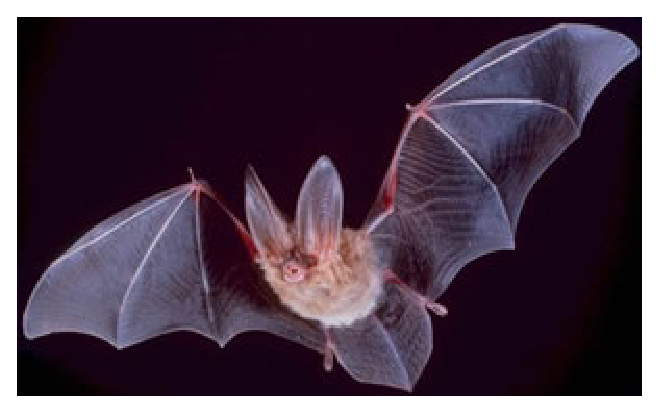
\includegraphics[width=.45\linewidth]{figs/bat_b.eps}\hspace*{0.04in}

\includegraphics[width=.36\linewidth]{figs/gull2_b.eps}\\
\end{center}
\vspace{-.1in}

\caption
{
Note how a picture that was created or imported differently has a different
space between caption and image than the line drawing in Figure
\protect\ref{pg1}. (Left) Bat flight is being studied as part of an
Air Force Office of Scientific Research Multidisciplinary
University Research Initiative project.
Image credit: mime.oregonstate.edu/news/story/2103, (Right)
Morphing gull wings.
{\em Note how the URL spills too far to the right in the
list of figures. This type of margin infraction must be
corrected manually.}}
%\end{singlespace}
\label{batgull2}
\end{figure}



Note that imported pictures that have white space on their margins
will look
as if they are placed incorrectly. For such pictures,
make a note on the printout that goes to format checking.



\section{Tables}

Tables pretty much act like figures.
I have little experience with them, but
Table \ref{tablelabel}
is an example.


\begin{table}[h]

\ \\

\caption{A sample table. If there are no tables,
comment out the $\setminus $include$\{ $tables$\} $ command in
phd\underline{~}thesis.tex.
{\em Note how the "include" spills too far to the right in the
list of figures. This type of margin infraction must be
corrected manually.}
}
\label{tablelabel}

\ \\

\centerline{
\begin{tabular}{|l|l|r|}
\hline
$p$ & $q$ & $p\Rightarrow q$ \\
\hline
F   & F   & T \\
\hline
F   & T  & T \\
\hline
T  & F   & F  \\
\hline
T  & T  & T  \\
\hline
\end{tabular}
}

\ \\
\vspace{-.1in}

\end{table}


For tables, the title is to be placed above the table,
which is done by putting the $\setminus $caption command
above the table.
To get a double space between the caption and the table,
place a ``$\setminus \ \setminus \setminus $"
on a line between the caption and the table.
To put a triple space between the title and the text above it,
place a ``$\setminus \ \setminus \setminus $"
on a line between the start of the table and the caption.
To put a triple space between the table and the text below it,
place a ``$\setminus \ \setminus \setminus $"
on a line after the end of the table,
but before the $\setminus $end$\{ $table$\} $ command.





\begin{table}[h]

\ \\
\vspace{-.15in}

\caption{Another sample table and another fun rule:
Entries in the list of tables/figures
should have at least 3 dots in the dotted
line between entry and page number. Unless there is
an unfortunate spill, which would need to be fixed anyway,
\LaTeX \ should do this automatically.
}
\label{tablelabel2}

\ \\

\centerline{
\begin{tabular}{|l|l|r|}
\hline
$p$ & $q$ & $p\Rightarrow q$ \\
\hline
F   & F   & T \\
\hline
F   & T  & T \\
\hline
T  & F   & F  \\
\hline
T  & T  & T  \\
\hline
\end{tabular}
}

\end{table}


\addtocontents{lot}{So the entries above would need to be fixed by
rewording to eliminate the spills.
(And entries like this one are not permissible.)
\\
~\\
}

\addtocontents{lot}{Also note that to
shrink the gap between the dotted line and the
end of the entry, you should put the closing parenthesis
$\} $ of the caption command right after the last work of the
caption, not on the next line. Compare the entries for
Table \protect\ref{tablelabel} (bad)
and for Figure \protect\ref{batgull2} on the next page.
}


\section{Note on Sections}

If a chapter has only one section, omit the sectioning command.
So for this chapter, I had the choice to omit the section heading
``table" or to explain the reasoning in this short ``section."
